\section{Technical Description}
\label{sec:technical}

To find useful \emph{tap points} in a system---places from which to
extract data for introspection---using Tappan Zee Bridge, one begins by
creating a recording that captures the desired OS or application
behavior. For example, if the end goal is to be notified each time a
user loads a new URL in Firefox, one would create a recording of Firefox
visiting several URLs. This recording is made by emulating the OS and
application inside of TZB, which can capture and record all sources of
non-determinism with low overhead, allowing for later deterministic
replay. Next, one can run one or more analyses that seek out the desired
information among all memory accesses seen during the execution.
Analyses in TZB take the form of plugins that are called on each memory
access made during a replayed execution and, at the end, write out a
report on the tap points analyzed. Finally, the tap points found should
be validated to ensure that they do, in fact, provide the desired
information. Such assurance can be gained either by examining the data
in the tap point in new executions, or by examining the code around the
tap point. This workflow is illustrated in Figure~\ref{fig:workflow}.

In this section, we give a technical description of Tappan Zee Bridge.
We begin by giving a precise definition of a tap point, and discuss the
implications of our choice of definition. Next, we describe three
different ways of finding tap points: searching for ``known knowns'' ---
tap points where the desired data and its format is known; searching for
``known unknowns'' --- tap points where the kind of data sought is known,
but its precise format is not; and finally ``unknown unknowns'' --- tap
points where the type and format of the data sought are not known, and
we are instead simply trying to find ``interesting'' tap points.

\subsection{Defining Tap Points}

\begin{figure}[t]
\begin{center}
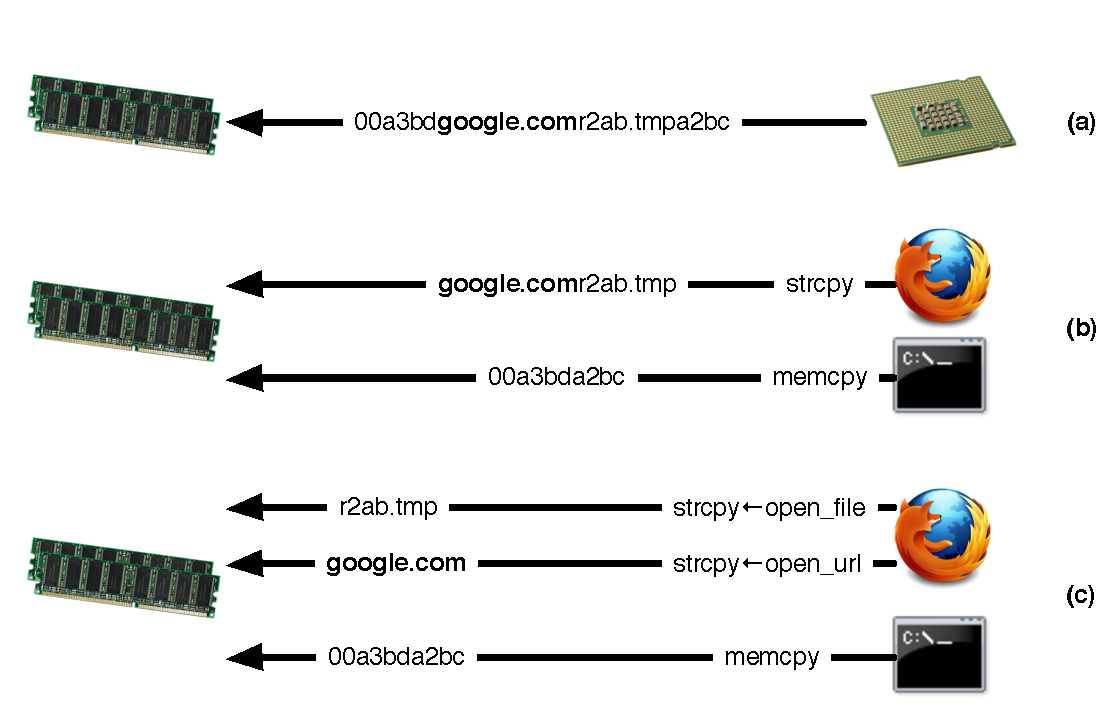
\includegraphics[width=3.2in]{tappoint.pdf}
\end{center}
\caption{Three different ways of defining a tap point: (a) as a single
stream of information from the CPU to RAM ; (b) split up according to
program and location within program ; (c) split up according to program,
location within program, and calling context.}
\label{fig:tappoint}
\end{figure}

A naive approach to defining tap points would be to simply group memory
accesses by the program counter that made them (e.g., EIP/RIP on x86 and
R15 on ARM). However, this approach fails in two common cases: first,
memory accesses made by bulk copy functions, such as \texttt{memcpy} and
\texttt{strcpy}, would all be grouped together, which would commingle
data from different parts of the program into the same tap point. In
addition, looking only at the program counter would conflate accesses
from different programs.

Instead, we define tap points as the triple \[ (caller, program\_counter,
address\_space) \] Including the caller and the address space (the
\texttt{CR3} register on x86, and the \fixme{register} on ARM) separates
out memory accesses into streams that should, in general contain the
same type of data. Figure \ref{fig:tappoint} shows the effect of
choosing various definitions of a tap point when looking for the place
where the browser writes the URL entered by the user (``google.com'').
At the coarsest granularity (a), one can simply look at all writes from
the CPU to RAM; however, the desired information is buried among reams
of irrelevant data. Separating out tap points by program and program
counter (b) is better, but still combines uses of \texttt{strcpy} that
contain different information --- in this case, a filename and a URL. By
including the calling context (c), we can finally obtain a tap point
that contains just the desired information.

Collecting information about the caller is accomplished in TZB in an
architecture-specific way. On 32-bit x86, we simply read the return
address off the stack. Aside from a small number of functions which are
optimized using frame pointer omission, this reliably gets the call site
for the current function. On other architectures, where stack-walking is
unreliable, we can run a pass that constructs a shadow stack based on
function calls and returns, which allows us to generically obtain an
accurate call stack at all times, but takes extra time up-front to
compute.

Although it is possible that some tap points may require deeper
information about the calling context (for example, if an application
has its own wrapper around \texttt{memcpy}), we have found that just one
level of calling context is usually sufficient. In addition, because TZB
is a whole-system emulator that can watch every call and return, we can
obtain the call stack to an arbitrary depth for any tap point. This
makes it easy to add extra context for a given tap point, if it is found
that doing so separates out the desired information.

\fixme{Might need to cut this paragraph since we haven't tested the tap
point correlation stuff.} Conversely, one might wonder whether this
definition of a tap point may split up data that should logically be
kept together. To address this case, we introduce the idea of
\emph{correlated tap points}: we can run a pass over the recorded
execution that notices when two tap points write to adjacent locations
in memory. The idea is that these tap points may be more usefully
considered jointly; for example, a single data structure may have its
fields set by successive writes. These writes would come from different
program counters, and hence would be split into different tap points,
but it may be more useful to examine the data structure as a whole. By
noticing this correlation we can analyze the data from the combined tap
point.

\subsection{Known Knowns}

The simplest case is finding data that one knows is likely to be read or
written by a tap point, and where the encoding of the data is easily
guessed. For example, to find a tap point that can be used to notify
the hypervisor whenever a URL is entered in a browser, one can visit a
known sequence of URLs, and then monitor all tap points, searching for
specific byte sequences that make up those URLs. The same holds for
other data whose representation when written to memory is predictable:
filenames, window titles, registry key names, and so on.

To realize this in TZB, we developed a plugin (\texttt{stringsearch})
that can quickly search for byte strings read or written by tap points
during a recorded execution. This can be accomplished with low overhead:
for each string sought and each tap point, we simply keep a counter that
tracks how many characters of the string have been matched so far, and
reset the counter as soon as a non-matching character is found. If this
counter ever equals the length of the string, then we can conclude that
the tap point has read or written the desired information.

\subsection{Known Unknowns}
\label{sec:technical:subsec:knownunk}

A second tap point application involves finding tap points for things
about which we have limited knowledge.

We can easily assemble corpora of exemplars to represent a semantic
class: English prose, kernel messages, or mail headers. These examples
need not come from tap points but can easily be collected directly from
interacting with the operating system itself. From such a corpus, we can
readily build a statistical model of the semantic class. Tap points
whose contents have high likelihood ratios for the semantic model with
respect to a null model are likely to come from the same semantic class
as the corpus. This kind of supervised learning permits us, for
instance, to train a model on examples of the contents of \texttt{dmesg}
under Linux and employ it to locate tap points that write analogous data
in other operating systems such as FreeBSD, Minix, and Haiku.

In TZB, we accomplish this by collecting bigram statistics for all tap
points seen in execution, as well as for the exemplar; the data seen at
each tap point is thus represented as a sparse vector with 65,536
elements (one for each possible pair of bytes). We can then sort the tap
points seen by taking the distance (according to some metric) from the
exemplar. For our metric, we have chosen cosine similarity, which gives
better results than Euclidean distance on high-dimensional, sparse data.
It can also be efficiently implemented in terms of sparse matrix
operations, which is helpful, since we are typically dealing with
millions of tap points. Cosine similarity for two vectors $u$ and $v$ is
defined as:

\[
1 - \frac{u \cdot v}{||u||_2 ||v||_2}
\]

\noindent where $||u||_2$ is defined as the $l^2$-norm of $u$.

In addition to statistical comparison to a known exemplar, we can also
search for data of unknown format if we have access to some external
validator. This is the case, for example, when searching for tap points
that write encryption keys: although the exact key may not be known in
advance (ruling out the use of the \texttt{stringsearch} plugin), if we
have bit of encrypted data we can check whether a given byte string is a
valid decryption key.

In TZB, we currently implement this strategy for finding tap points that
write SSL/TLS master secrets, the 48-byte strings from which an
SSL/TLS-encrypted session's keys are derived. In the training phase, we
record the execution of a program that initiates an encrypted connection
to some server; we also record the encrypted packets sent by the client.
Then, using the \texttt{keyfind} plugin, we test each 48 bytes written
by each tap point and see whether the keys derived from it successfully
decrypt a sample packet sent by the client. If so, then we conclude that
the tap point can be used to decrypt SSL/TLS connections made by the
program under inspection. In Section~\ref{sec:eval:subsec:sslmal} we show
how this technique can be used to spy on connections made by the Sykipot
malware, without performing a (potentially detectable) man in the middle
attack.

\subsection{Unknown Unknowns}

The final strategy for finding useful tap points is also the least
focused. If there is no specific introspection quantity sought, one
might instead wish to find interesting tap points, for some suitable
definition of ``interesting.'' To support this scenario, TZB offers a
form of unsupervised learning---clustering---to group together tap
points that handle similar data. The idea is that one can then examine
exemplars from each cluster, rather than being forced to look through a
large number of tap points. Thus, our use of clustering functions as a
form of \emph{data triage}.

Our clustering is based on the venerable $k$-means
algorithm~\cite{Steinhaus:1956kx}, but using the cosine distance measure
described in the previous section. This variant of $k$-means is known as
\emph{spherical $k$-means}.~\cite{Dhillon:2001fk} As in the statistical
search case, we use bigram statistics for our feature vectors, and we
weight each vector using the well-known ``term frequency-inverse
document frequency''~\cite{Sparck-Jones:1988uq} statistic from
information retrieval, which helps increase the effect of rare bigrams
for distinguishing between different tap points. We evaluate the
performance of this clustering compared to an expert labeling in
Section~\ref{sec:eval:subsec:cluster}.
